%% -*- mode: LaTeX; TeX-master: "../Summer14.tex" -*-
%% ///////////////////////////////////////////////////////////////////////////
\ifhevea
\tausection{Combination of upper limits on \mtau LFV branching fractions: summary plot}
\cutname{lfv-combinations-plot.html}
\fi

\begin{figure}[tb]
  \begin{center}
    \ifhevea
    \begin{tabular}{@{}cc@{}}
      \larger\bfseries\ahref{TauLFV_UL_2014001_averaged.png}{full size PNG} &
      \larger\bfseries\ahref{TauLFV_UL_2014001_averaged.pdf}{PDF format} \\
      \multicolumn{2}{c}{\ahref{TauLFV_UL_2014001_averaged.png}{%
          \imgsrc[alt="Tau LFV limits combinations plot" width=720]{TauLFV_UL_2014001_averaged.png}}}
    \end{tabular}
    \else
    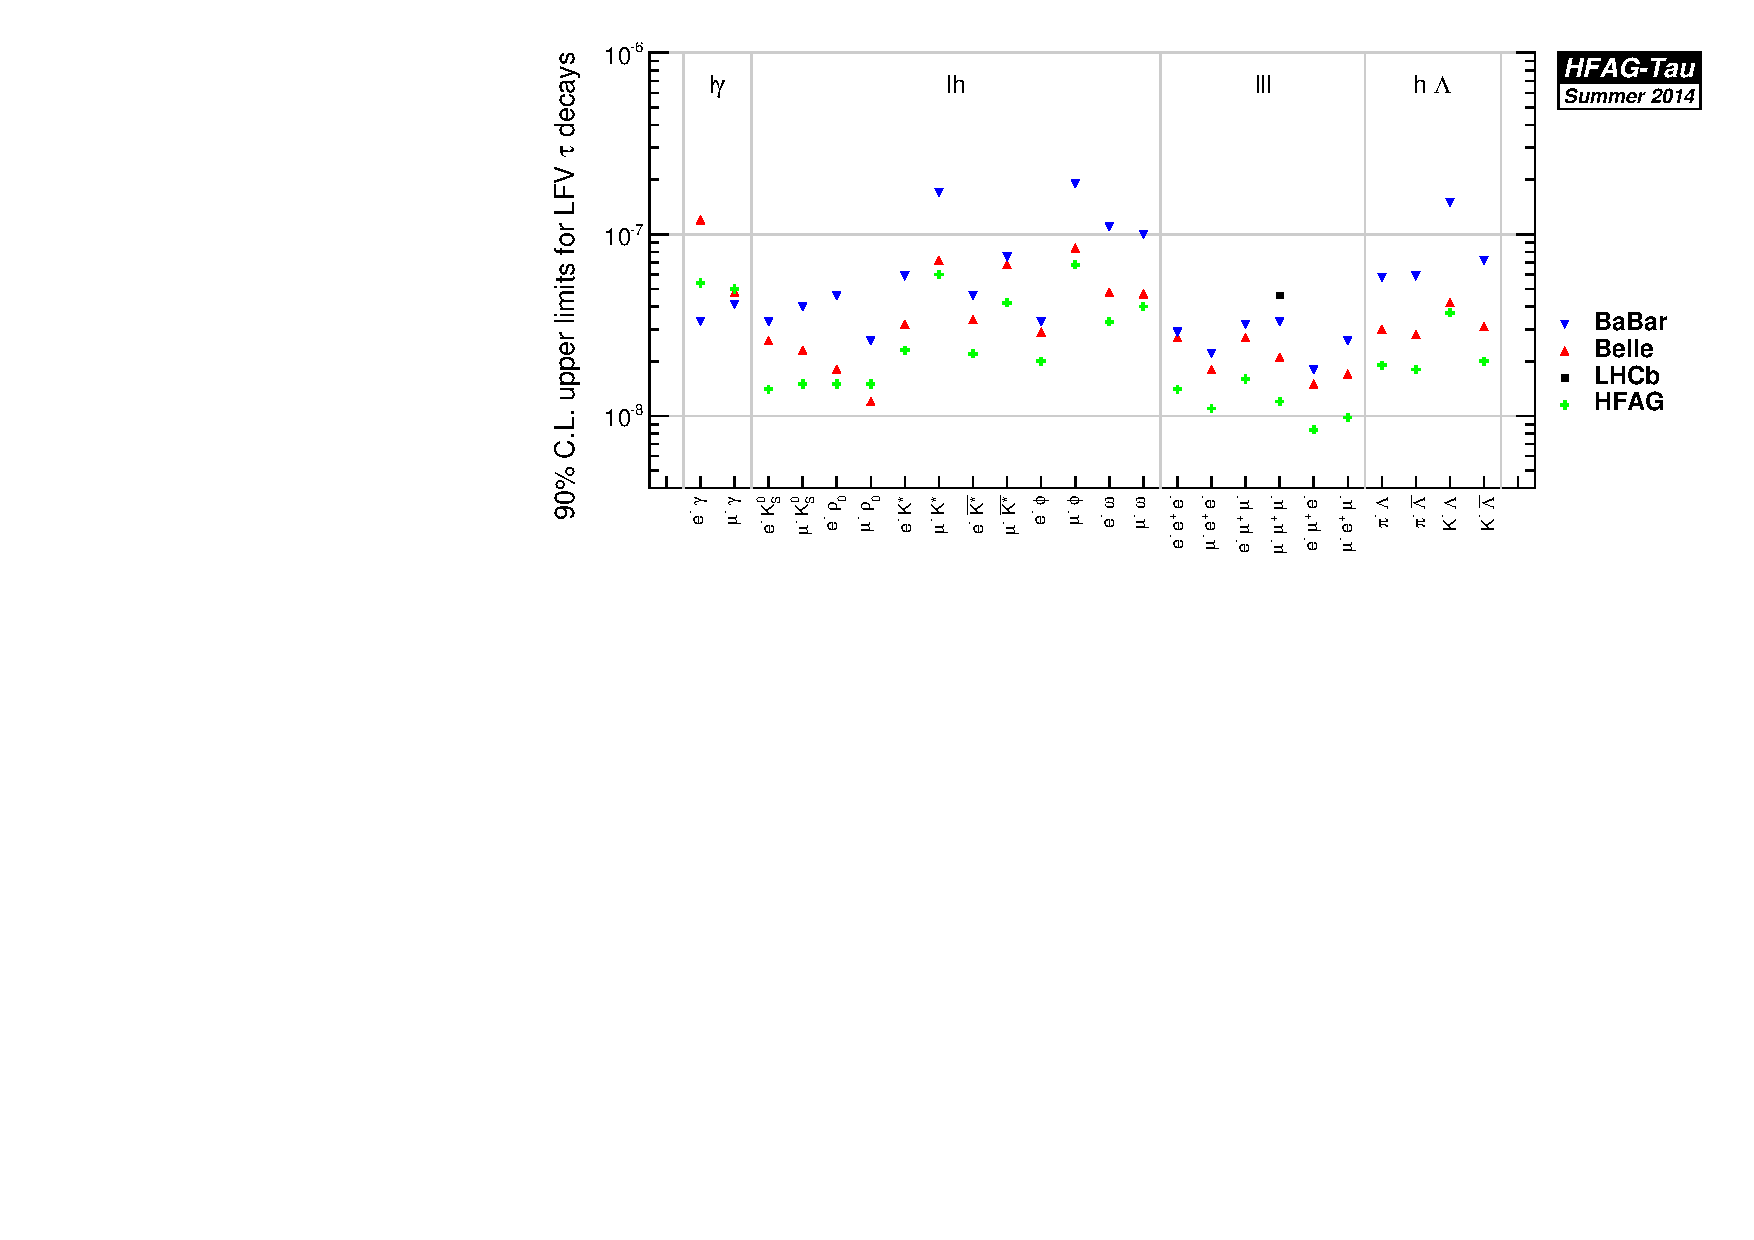
\includegraphics[angle=270,totalheight=0.86\textheight,clip]{figures/tau/TauLFV_UL_2014001_averaged.pdf}
    \fi
    \caption{Tau lepton-flavour-violating branching fraction upper limits
      combinations summary plot. For each channel we report the HFAG
      combined limit, and the experimental published limits. In some cases,
      the combined limit is weaker than the limit published by a single
      experiment. This arises since the \cls method used in the
      combination can be more conservative compared to other legitimate
      methods, especially when the number of observed events fluctuates below the
      expected background. 
      \label{fig:tau:lfv-limits-plot-average}
    }
  \end{center}
\end{figure}
